\documentclass{article}
\usepackage{geometry}
\usepackage{titling}
\usepackage{hyperref}
\usepackage{amsmath}
\usepackage{amssymb}
\usepackage{graphicx}
\usepackage{caption}
\usepackage{subcaption}
\usepackage[dvipsnames]{xcolor}

\geometry{
  a4paper,
  total = {170mm, 257mm},
  left = 20mm,
  top = 20mm,
}
\graphicspath{ {./images/} }

\title{Trabajo práctico N° 4}
\author{Emanuel Nicolás Herrador}
\date{Abril 2025}

\makeatletter
\def\@maketitle{%
  \newpage
  \null
  \vskip 1em%
  \begin{center}%
  \let \footnote \thanks
    {\LARGE \@title \par}%
    \vskip 1em%
    {\large \@date}%
  \end{center}%
  \par
  \vskip 1em}
\makeatother

\begin{document}

\maketitle

\noindent\begin{tabular}{@{}ll}
	Estudiante & \theauthor \\
\end{tabular}

\section*{Ejercicio 2}
Veamos cada una por separado.
Comencemos con $\square\square\varphi \to \square\varphi$.
Notemos que por definición tenemos lo siguiente:
\begin{equation*}
	\begin{aligned}
		\sigma \vDash \square\square\varphi & \iff \forall j \geq 0 : \sigma[j..] \vDash \square\varphi                      \\
		                                    & \iff \forall j \geq 0 : \forall j_2 \geq 0 : \sigma[j..][j_2..] \vDash \varphi \\
		                                    & \iff \forall i \geq 0 : \sigma[i..] \vDash \varphi                             \\
		                                    & \iff \sigma \vDash \square\varphi
	\end{aligned}
\end{equation*}
Luego, es trivial que se verifica la implicación porque son fórmulas equivalentes.

Para $\square(\varphi \land \psi) \to \square\varphi \land \square\psi$ veamos que:
\begin{equation*}
	\begin{aligned}
		\sigma \vDash \square(\varphi \land \psi) & \iff \forall j \geq 0 : \sigma[j..] \vDash \varphi \land \psi                                               \\
		                                          & \iff \forall j \geq 0 : \sigma[j..] \vDash \varphi \land \sigma[j..] \vDash \psi                            \\
		                                          & \iff (\forall j \geq 0 : \sigma[j..] \vDash \varphi) \land (\forall j_2 \geq 0 : \sigma[j_2..] \vDash \psi) \\
		                                          & \iff \sigma \vDash \square\varphi \land \sigma \vDash \square\psi                                           \\
		                                          & \iff \sigma \vDash \square\varphi \land \square\psi
	\end{aligned}
\end{equation*}
Con ello, resulta trivial la implicación al ser fórmulas equivalentes.

Y, por último, queda ver que $\diamondsuit(\varphi \lor \psi) \to \diamondsuit\varphi \lor \diamondsuit\psi$:
\begin{equation*}
	\begin{aligned}
		\sigma \vDash \diamondsuit(\varphi \lor \psi) & \iff \exists j \geq 0 : \sigma[j..] \vDash (\varphi \lor \psi)                                             \\
		                                              & \iff \exists j \geq 0 : \sigma[j..] \vDash \varphi \lor \sigma[j..] \vDash \psi                            \\
		                                              & \iff (\exists j \geq 0 : \sigma[j..] \vDash \varphi) \lor (\exists j_2 \geq 0 : \sigma[j_2..] \vDash \psi) \\
		                                              & \iff \sigma \vDash \diamondsuit\varphi \lor \sigma \vDash \diamondsuit\psi                                 \\
		                                              & \iff \sigma \vDash (\diamondsuit\varphi \lor \diamondsuit\psi)
	\end{aligned}
\end{equation*}
Luego, al ser equivalentes, claramente se cumple la implicación.

\section*{Ejercicio 3}
Ver la validez de la fórmula equivale a ver si se cumple la equivalencia dada por $\square(p \land \diamondsuit q) \equiv \square(p \text{U} q)$.
Para ello, una forma de refutar la validez es mostrar una traza que cumple una propiedad pero la otra no.
Veamos que $(\{q\})^\omega$ cumple claramente $\square(p \text{U} q)$ pero no $\square(p \land \diamondsuit q)$.
Luego, se refuta. $\blacksquare$

\section*{Ejercicio 4}
Se pretende demostrar formalmente que \textit{strong fairness} implica \textit{weak fairness}.
Es decir, es quiere ver que $(\square\diamondsuit\varphi \to \square\diamondsuit \psi) \to (\diamondsuit\square\varphi \to \square\diamondsuit\psi)$.

Para ello, expandamos cada una de las partes:
\begin{equation*}
	\begin{aligned}
		\square\diamondsuit\varphi \to \square\diamondsuit\psi & \equiv \neg\square\diamondsuit\varphi \lor \square\diamondsuit\psi \\
		\diamondsuit\square\varphi \to \square\diamondsuit\psi & \equiv \neg\diamondsuit\square\varphi \lor \square\diamondsuit\psi
	\end{aligned}
\end{equation*}

Ahora, supongamos que \textit{strong fairness} vale para un $\sigma$ dado que $\sigma \vDash \square\diamondsuit\psi$.
Luego, es claro que, por la anterior expansión, también vale \textit{weak fairness} para $\sigma$.

En caso de que valiera \textit{strong fairness} pero solo porque $\sigma \vDash \neg\square\diamondsuit\varphi$, podemos notar lo siguiente:
\begin{equation}
	\tag*{(4.1)}
	\begin{aligned}
		\sigma \vDash \neg\square\diamondsuit\varphi & \iff \neg(\forall i \geq 0 : \exists j \geq 0 : \sigma[i..][j..] \vDash \varphi) \\
		                                             & \iff \exists i \geq 0 : \forall j \geq 0 : \sigma[i..][j..] \vDash \neg\varphi   \\
		                                             & \iff \exists i \geq 0 : \forall j \geq i : \sigma[j..] \vDash \neg\varphi        \\
	\end{aligned}
\end{equation}

Ahora, nuestro objetivo es llegar a $\sigma \vDash \neg\diamondsuit\square\varphi$, lo cual significa que:
\begin{equation}
	\tag*{(4.2)}
	\begin{aligned}
		\sigma \vDash \neg\diamondsuit\square\varphi & \iff \neg(\exists i \geq 0 : \forall j \geq 0 : \sigma[i..][j..] \vDash \neg\varphi) \\
		                                             & \iff \forall i \geq 0 : \exists j \geq 0 : \sigma[i..][j..] \vDash \neg\varphi       \\
		                                             & \iff \forall i \geq 0 : \exists j \geq i : \sigma[j..] \vDash \neg\varphi
	\end{aligned}
\end{equation}

Si $\sigma \vDash \neg\square\diamondsuit\varphi$, entonces por $(4.1)$ es de la forma $(\emptyset + \{\varphi\} + \{\psi\} + \{\varphi, \psi\})^*(\emptyset + \{\psi\})^\omega$.
Con ello, claramente $\sigma \vDash \neg\diamondsuit\square\varphi$ por $(4.2)$ porque sea $j$ el índice más chico a partir del cual todo elemento de la traza cumple $\neg\varphi$, entonces $\forall 0 \leq i \leq j : \sigma[j..] \vDash \neg\varphi$ y $\forall j \leq i : \sigma[i..] \vDash \neg\varphi$.

Por esto, se demuestra por completo que \textit{strong fairness} implica \textit{weak fairness} dado que si una traza satisface la primera, entonces también satisfará la segunda. $\blacksquare$

\section*{Ejercicio 5}
Veamos cada una:
\begin{itemize}
	\item ``Si $\varphi$ es cierto durante la ejecución del programa, eventualmente ocurrirá $\psi$'': $\square(\varphi \to \diamondsuit\psi)$.
	\item ``No es posible que $\varphi$ y $\psi$ ocurran simultáneamente durante la ejecución del programa'': $\neg\diamondsuit(\varphi \land \psi)$.
	\item ``Cada vez que $\varphi$ sea cierto, $\psi$ también lo es'': $\square(\varphi \to \psi)$.
	\item ``$\varphi$ no deja de ocurrir, al menos hasta que $\psi$ ocurra'': $\varphi \text{WU} \psi \equiv \square\varphi \lor (\varphi \text{U} \psi)$.
\end{itemize}

\section*{Ejercicio 6}
Se define el operador \textit{while} como:
\begin{equation*}
	\tag*{(6.1)}
	\sigma \vDash \varphi \text{W} \psi \iff \forall i \geq 0 : (\forall 0 \leq j \leq i : \sigma[j..] \vDash \psi) \Rightarrow \sigma[i..] \vDash \varphi
\end{equation*}

Para poder resolver los siguientes items de este ejercicio, va a ser útil desglosar la definición para entenderla a detalle.
Tomemos la definición de $(6.1)$ y digamos que tenemos un $x$ tal que $\forall 0 \leq j \leq x : \sigma[j..] \vDash \psi$.
Ahora, por la definición, sabemos que $\sigma[x..] \vDash \varphi$.
Además, es trivial notar que $\forall 0 \leq j \leq x-1 : \sigma[j..] \vDash \psi$, por lo que por definición $\sigma[(x-1)..] \vDash \varphi$.
Expandiendo esta idea, llegamos a que $\forall 0 \leq j \leq x : \sigma[j..] \vDash \varphi$.

Con lo anterior, la definición puede pasar a ser:
\begin{equation*}
	\tag*{(6.2)}
	\sigma \vDash \varphi \text{W} \psi \iff \forall i \geq 0 : (\forall 0 \leq j \leq i : \sigma[j..] \vDash \psi) \Rightarrow (\forall 0 \leq j \leq i : \sigma[j..] \vDash \varphi)
\end{equation*}

El \textbf{primer punto} solicita expresar el operador \textit{while} en términos del \textit{until} y expresiones booleanas.
Para ello, podremos pensar que siempre en el prefijo se cumple $\psi \to \varphi$ hasta que deja de cumplirse $\psi$.
Es decir: $\varphi \text{W} \psi \equiv ((\psi \to \varphi) \text{U} \neg\psi) \lor \square(\psi \land \varphi)$.
Lo único a modificar es el \textit{globally}, el cual se puede considerar como $\neg (\text{T}\ \text{U} \neg (\psi \land \varphi))$ donde $T$ es una tautología.
Notar que en este caso se busca que no se cumpla que en algún momento suceda $\neg (\psi \land \varphi)$.
Por ello, decimos que: $\varphi \text{W} \psi \equiv ((\psi \to \varphi) \text{U} \neg\psi) \lor \neg(\text{T}\ \text{U} \neg(\psi \land \varphi))$.

Finalmente, el \textbf{segundo punto} pide expresar el operator \textit{until} en términos del \textit{while} y operaciones booleanas.
Aquí, como queremos que el until sea $\varphi \text{U} \psi$ y dada la definición vista anteriormente, tomaremos algo de la forma $\gamma \text{W} \neg\psi \land \diamondsuit\psi$.
De este modo, tendremos que $\gamma \text{W} \neg\psi \land \diamondsuit\psi \equiv (((\neg\psi \to \gamma) \text{U} \psi) \lor \square(\neg\psi \land \gamma)) \land \diamondsuit\psi$.
Como no puede cumplirse al mismo tiempo $\square(\neg\psi \land \gamma)$ y $\diamondsuit\psi$, tenemos que $\gamma \text{W} \neg\psi \land \diamondsuit\psi \equiv (\neg\psi \to \gamma) \text{U} \psi \land \diamondsuit\psi$.
Ahora, al ser un until, $\diamondsuit\psi$ resulta redundante dado que el until ya garantiza que en algún momento $\psi$ sucederá.
Por ello, podemos considerar $\gamma \text{W} \neg\psi \land \diamondsuit\psi \equiv (\neg\psi \to \gamma) \text{U} \psi$.
Finalmente, se busca que $\neg\psi \to \gamma \equiv \varphi$.
Si bien esto no es posible, podemos considerar $\gamma = \varphi$ tal que $\varphi \text{W} \neg\psi \land \diamondsuit\psi \equiv (\neg\psi \to \varphi) \text{U} \psi$.

Si bien este último punto es diferente al until que queremos, igualmente es válido dado que cuando valga por primera vez $\psi$ este marcará el final del until.
En las posiciones anteriores a este final, se cumplirá $\neg\psi$ por lo que el implica determina que vale $\varphi$ en cada paso anterior.
Por ello, finalmente, consideramos $\varphi \text{U} \psi \equiv \varphi \text{W} \neg\psi \land \diamondsuit\psi$.
El único paso que resta realizar es la traducción de $\diamondsuit\psi$ con el uso del \textit{while}.
Para ello, tenemos $\diamondsuit\psi \equiv \neg(\neg\psi \text{W T})$ dado que no se cumple que mientras suceda ``cualquier propiedad'' no se cumpla $\psi$.
Notar que el while aquí junto a la tautología ayuda a expresar el globally.
Finalmente, la equivalencia queda como $\varphi \text{U} \psi \equiv (\varphi \text{W} \neg\psi) \land \neg(\neg\psi \text{W T})$.

\section*{Ejercicio 7}
Queremos definir el operador $\text{Z}$ tal que $\varphi \text{Z} \psi$ represente la propiedad de que siempre entre dos posiciones distintas en las cuales valga $\varphi$, existe una en la que vale $\psi$.
Considero que estar entre medio de las otras dos implica que no se consideran los extremos.

Motivo de ello, la definición que doy es la siguiente: $\square(\varphi \to \neg\bigcirc(\neg\psi \text{U} \varphi))$.
Es decir, me concentro en la negación de la propiedad para definirla.
Considero que cuando ``veo'' un $\varphi$, entonces a partir de la siguiente posición no puede pasar que veo otro $\varphi$ antes de algún $\psi$.

\section*{Ejercicio 8}
Veamos cada autómata con alfabeto $\{a, b, c\}$ por separado.

Para el caso de conjunto de cadenas infinitas con una cantidad finita de $a$ tenemos el siguiente diagrama:
\begin{figure}[!htb]
	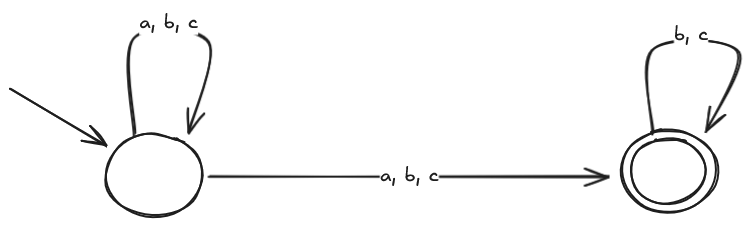
\includegraphics[width=0.7\textwidth]{04-08-a.png}
	\centering
\end{figure}

Para el conjunto de cadenas infinitas en que cada ocurrencia de $c$ viene inmediatamente seguida de una ocurrencia de $b$ tenemos:
\begin{figure}[!htb]
	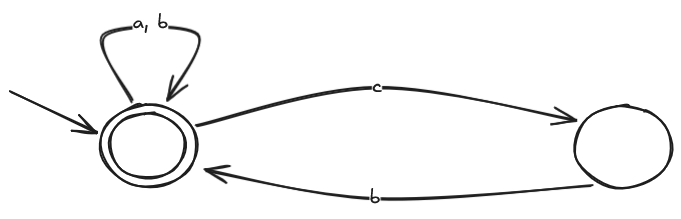
\includegraphics[width=0.7\textwidth]{04-08-b.png}
	\centering
\end{figure}

Para el conjunto de cadenas infinitas que no terminen en una secuencia infinita de $a$ ni en una de $b$ ni en una de $c$ tenemos:
\begin{figure}[!htb]
	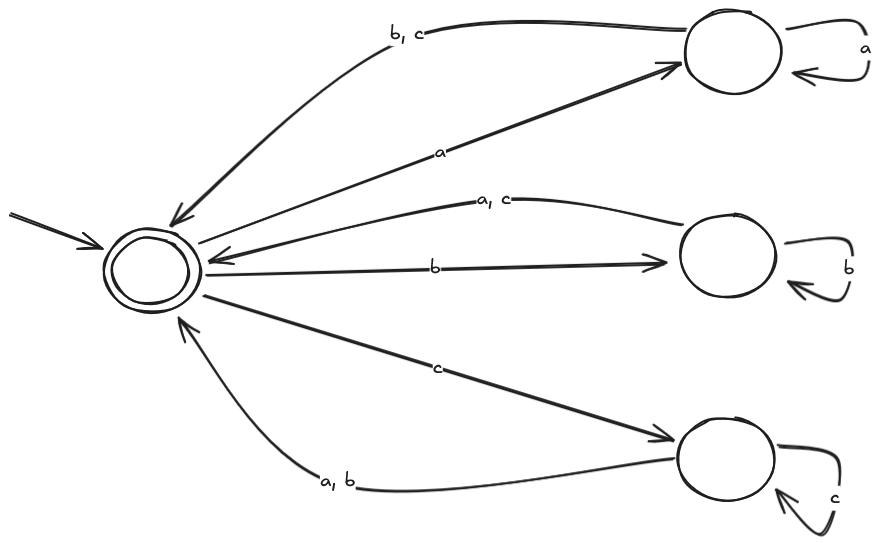
\includegraphics[width=0.7\textwidth]{04-08-c.png}
	\centering
\end{figure}

Y para el conjunto de cadenas infinitas con cantidades finitas de $a$, $b$ y $c$, como el alfabeto es $\{a, b, c\}$, entonces el conjunto es claramente vacío.
Por ello, el autómata de Büchi puede ser cualquiera siempre y cuando el conjunto de estados aceptados sea vacío.

\section*{Ejercicio 9}
Notemos que el diagrama de la izquierda representa el lenguaje $\omega$-regular $b^*a(a + b)^\omega$ mientras que el de la derecha a $(a + b)^*a(a + b)^\omega$.
Por ello, aceptan el mismo lenguaje $\omega$-regular porque el no determinismo de la transición $a$ en el autómata de la derecha se puede resolver tomando siempre la transición que conecta ambos estados.
Se puede verificar que esto no modifica el lenguaje del autómata porque en ambos estados puede tomar las mismas acciones, por lo que se sigue cumpliendo que toda traza con al menos una $a$ sea aceptada.

Respecto al lenguaje $\omega$-regular, como bien se dijo antes, es aquél que expresa que toda traza con al menos una $a$ es aceptada.
Por motivos de facilidad para notar el prefijo que se quiere, considero la expresión no determinística del autómata de la derecha.

\section*{Ejercicio 10}
Las expresiones $\omega$-regulares tratadas en los ejercicios 8, 9 y 10 de la anterior guía se presentan a continuación junto con el autómata de Büchi correspondiente:
\begin{figure}[!htb]
	\renewcommand\thesubfigure{\arabic{subfigure}}
	\centering
	\begin{subfigure}[b]{0.2\textwidth}
		\centering
		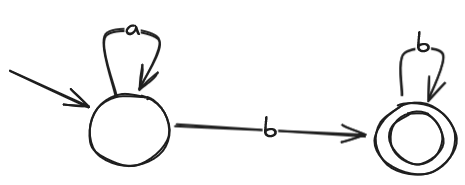
\includegraphics[width=\textwidth]{04-10-01.png}
		\caption{$a^*b^\omega$}
	\end{subfigure}
	\hfil
	\begin{subfigure}[b]{0.3\textwidth}
		\centering
		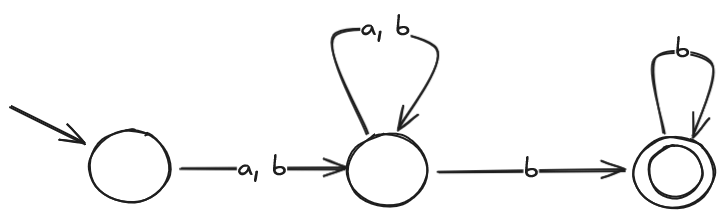
\includegraphics[width=\textwidth]{04-10-02.png}
		\caption{$(b + a)^+b^\omega$}
	\end{subfigure}
	\hfil
	\begin{subfigure}[b]{0.3\textwidth}
		\centering
		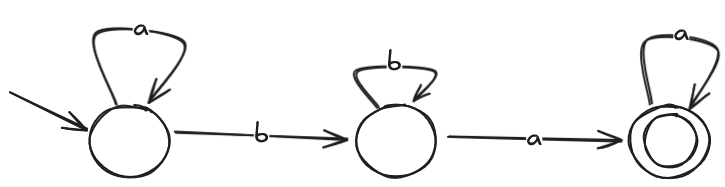
\includegraphics[width=\textwidth]{04-10-03.png}
		\caption{$a^*b^+a^\omega$}
	\end{subfigure}
	\hfil
	\begin{subfigure}[b]{0.3\textwidth}
		\centering
		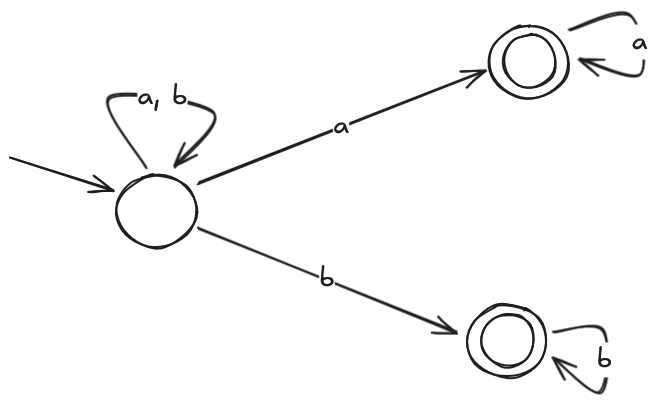
\includegraphics[width=\textwidth]{04-10-04.png}
		\caption{$(a + b)^*(a^\omega + b^\omega)$}
	\end{subfigure}
	\hfil
	\begin{subfigure}[b]{0.3\textwidth}
		\centering
		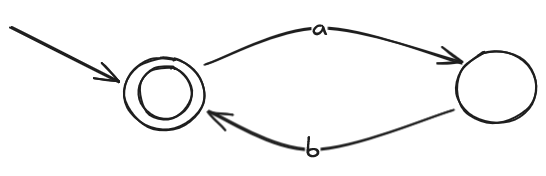
\includegraphics[width=\textwidth]{04-10-05.png}
		\caption{$(ab)^\omega$}
	\end{subfigure}
	\hfil
	\begin{subfigure}[b]{0.2\textwidth}
		\centering
		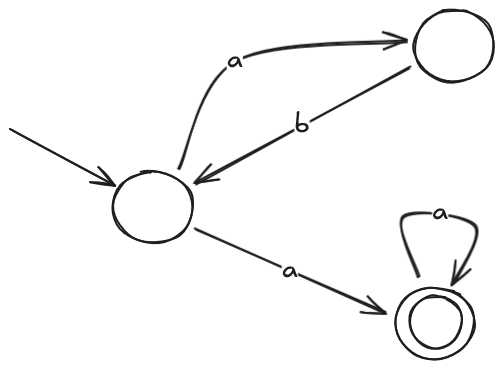
\includegraphics[width=\textwidth]{04-10-06.png}
		\caption{$(ab)^*a^\omega$}
	\end{subfigure}
	\hfil
	\begin{subfigure}[b]{0.2\textwidth}
		\centering
		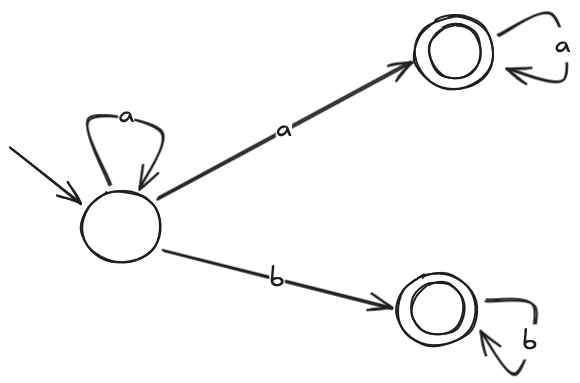
\includegraphics[width=\textwidth]{04-10-07.png}
		\caption{$a^*(a^\omega + b^\omega)$}
	\end{subfigure}
	\hfil
	\begin{subfigure}[b]{0.1\textwidth}
		\centering
		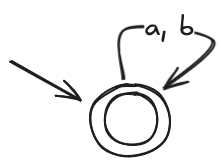
\includegraphics[width=\textwidth]{04-10-08.png}
		\caption{$\Sigma^\omega$}
	\end{subfigure}
	\hfil
	\begin{subfigure}[b]{0.4\textwidth}
		\centering
		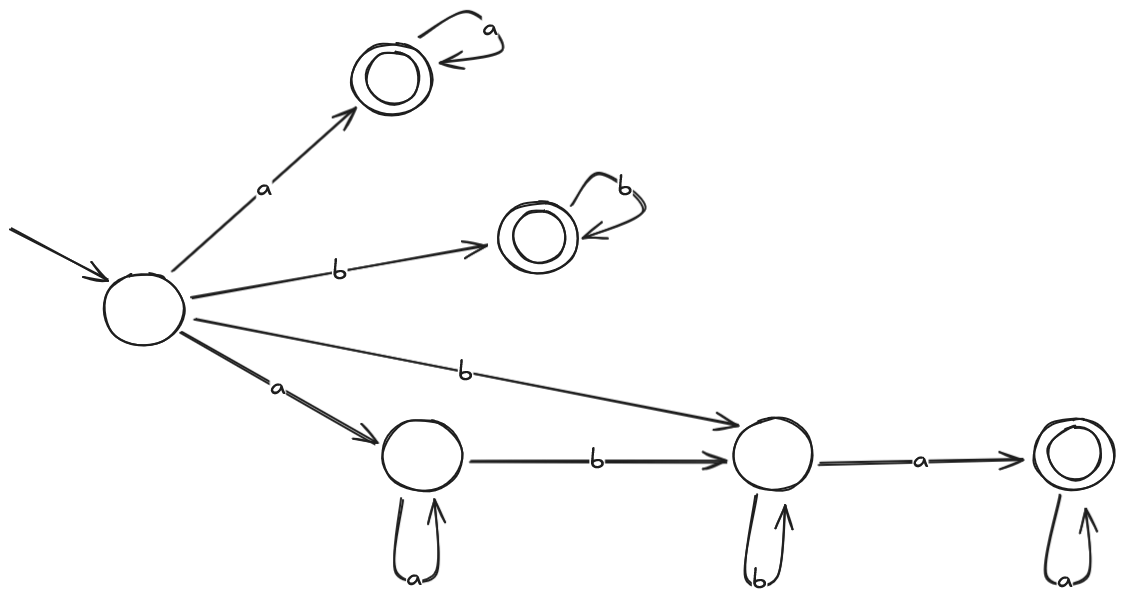
\includegraphics[width=\textwidth]{04-10-09.png}
		\caption{$a^*b^+a^\omega + a^\omega + b^\omega$}
	\end{subfigure}
	\hfil
	\begin{subfigure}[b]{0.3\textwidth}
		\centering
		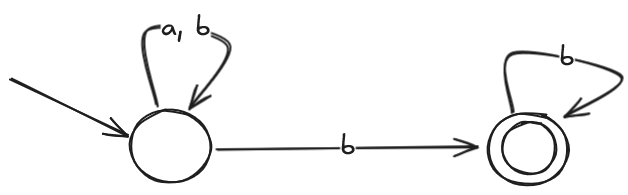
\includegraphics[width=\textwidth]{04-10-10.png}
		\caption{$(a^*b^\omega) + (a + b)^*b^\omega = (a + b)^*b^\omega$}
	\end{subfigure}
	\hfil
	\begin{subfigure}[b]{0.4\textwidth}
		\centering
		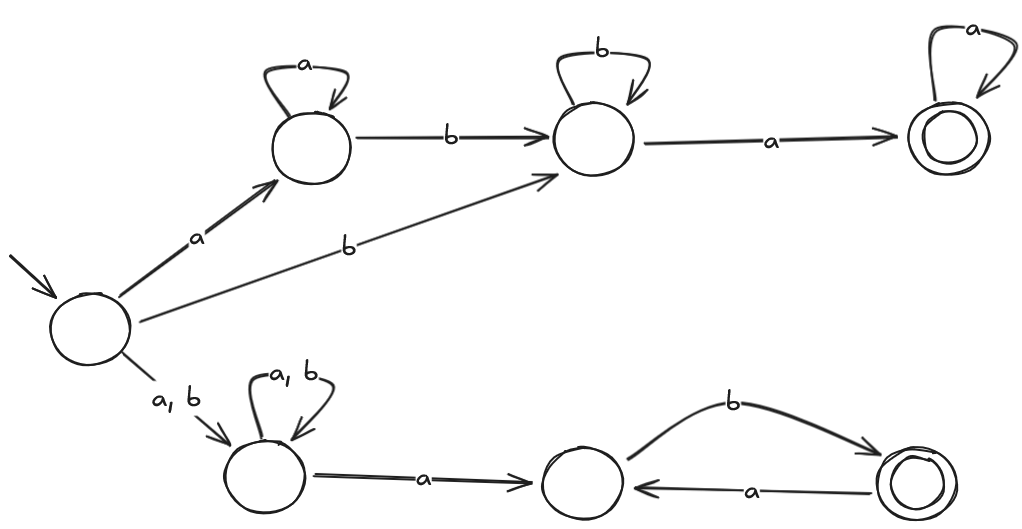
\includegraphics[width=\textwidth]{04-10-11.png}
		\caption{$a^*b^+a^\omega + (a + b)^*(ab)^\omega$}
	\end{subfigure}
	\hfil
	\begin{subfigure}[b]{0.35\textwidth}
		\centering
		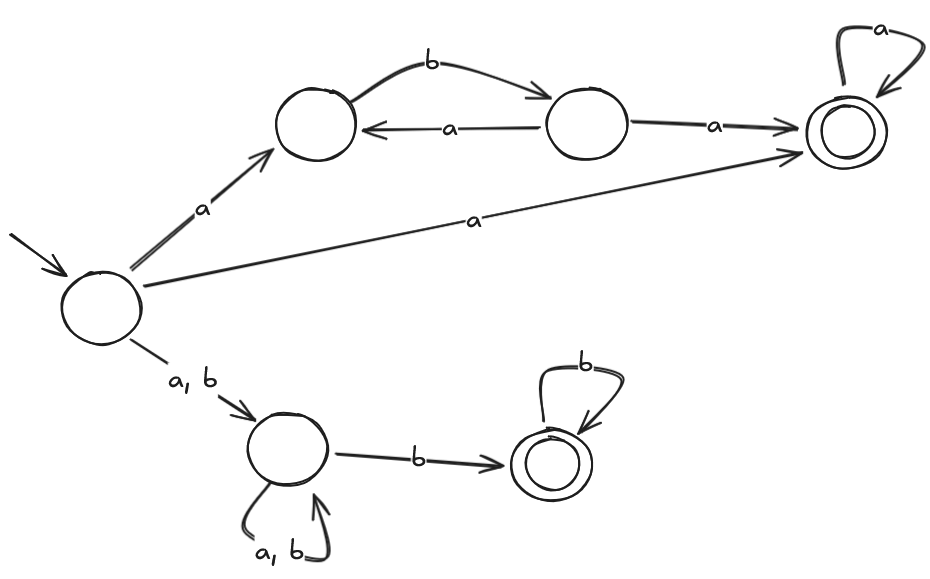
\includegraphics[width=\textwidth]{04-10-12.png}
		\caption{$(ab)^*a^\omega + (a + b)^*b^\omega$}
	\end{subfigure}
\end{figure}

\section*{Ejercicio 11}
Dados $\mathcal{A}_i = (S_i, s_0^i, \delta_i, \Sigma, A_i)$ con $i = 1, 2$ autómatas de Büchi, se define la intersección como:
\begin{equation*}
	\mathcal{A}_1 \cap \mathcal{A}_2 = (S_1 \times S_2 \times \{0, 1, 2\}, (s_0^1, s_0^2, 0), \delta, \Sigma, S_1 \times S_2 \times \{2\})
\end{equation*}
donde:
\begin{equation*}
	\begin{aligned}
		(s_1', s_2', i)                                           & \in \delta((s_1, s_2, j), a)                          \\
		                                                          & \Updownarrow                                          \\
		s_1' \in \delta_1(s_1, a) \land s_2' \in \delta_2(s_2, a) & \land \begin{cases}
			                                                                       & (j = 0 \land s_1 \in A_1 \land i = 1)    \\
			                                                                  \lor & (j = 0 \land s_1 \notin A_1 \land i = 0) \\
			                                                                  \lor & (j = 1 \land s_2 \in A_2 \land i = 2)    \\
			                                                                  \lor & (j = 1 \land s_2 \notin A_2 \land i = 1) \\
			                                                                  \lor & (j = 2 \land i = 0)
		                                                                  \end{cases}
	\end{aligned}
\end{equation*}

\section*{Ejercicio 12}
Se pretende demostrar la igualdad $\overline{L(A_\varphi)} = L(A_{\neg\varphi})$.
Para ello, sea $\sigma$ una traza, veamos que:
\begin{equation*}
	\begin{aligned}
		\sigma \in \overline{L(A_\varphi)} & \iff \sigma \notin L(A_\varphi)    \\
		                                   & \iff \sigma \notin L(\varphi)      \\
		                                   & \iff \sigma \not\vDash \varphi     \\
		                                   & \iff \sigma \vDash \neg\varphi     \\
		                                   & \iff \sigma \in L(\neg\varphi)     \\
		                                   & \iff \sigma \in L(A_{\neg\varphi})
	\end{aligned}
\end{equation*}

Luego, como $\forall \sigma : \sigma \in \overline{L(A_\varphi)} \iff \sigma \in L(A_{\neg\varphi})$, se demuestra la igualdad de los lenguajes.

\section*{Ejercicio 13}
Sea $\varphi$ una fórmula, se pretende dar un algoritmo para corroborar que sea satisfactible, es decir, si es verdadera en algún modelo.

Para ello, notemos que:
\begin{equation*}
	\begin{aligned}
		\varphi \text{ es satisfactible} & \iff \exists \sigma : \sigma \vDash \varphi           \\
		                                 & \iff \exists \sigma : \sigma \in \mathcal{L}(\varphi) \\
		                                 & \iff \mathcal{L}(\varphi) \neq \emptyset              \\
		                                 & \iff \mathcal{L}(\mathcal{A_\varphi}) \neq \emptyset
	\end{aligned}
\end{equation*}

Luego, entonces, el algoritmo se reduce a:
\begin{enumerate}
	\item Construir el autómata de Büchi de $\varphi$.
	\item Calcular el lenguaje de $\mathcal{A}_\varphi$.
	\item Corroborar la no vacuidad en el lenguaje.
\end{enumerate}

\section*{Ejercicio 14}
Se pretende dar un algoritmo que corrobore si un modelo $M$ refina a otro modelo $M'$, es decir, si todas las propiedades que $M$ satisface también las satisface $M'$.

Para ello, notemos que:
\begin{equation*}
	\begin{aligned}
		(\forall \varphi : M \vDash \varphi \Rightarrow M' \vDash \varphi) & \iff \mathcal{L}(M) \subseteq \mathcal{L}(M')                                             \\
		                                                                   & \iff \mathcal{L}(M) \cap \overline{\mathcal{L}(M')} = \emptyset                           \\
		                                                                   & \iff \mathcal{L}(\mathcal{A}_M) \cap \overline{\mathcal{L}(\mathcal{A}_{M'})} = \emptyset \\
		                                                                   & \iff \mathcal{L}(\mathcal{A}_M) \cap \mathcal{L}(\mathcal{A}_{M'}^c) = \emptyset
	\end{aligned}
\end{equation*}

Luego, entonces, el algoritmo se reduce a:
\begin{enumerate}
	\item Construir el autómata de Büchi de $\mathcal{A}_M$.
	\item Construir el autómata complemento de Büchi $\mathcal{A}^c_{M'}$.
	\item Calcular los lenguajes $\mathcal{L}(\mathcal{A}_M)$ y $\mathcal{L}(\mathcal{A}^c_{M'})$.
	\item Corroborar vacuidad en la intersección de los lenguajes.
\end{enumerate}

\section*{Ejercicio 15}

\subsection*{Item 1}
Se busca representar la propiedad de safety del problema de lectores-escritores.
Para ello, notar que se puede expresar positivamente como:
\begin{equation*}
	\square((\text{reader} > 0 \land \text{writer} = 0) \lor (\text{reader} = 0 \land \text{writer} \leq 1))
\end{equation*}
o, de forma más compacta e intuitiva, en su forma negativa:
\begin{equation*}
	\neg\diamondsuit(\text{reader} > 0 \land \text{writer} > 0)
\end{equation*}

\subsection*{Item 2}
Se busca representar, ahora, fairness incondicional en el problema de lectores y escritores.
Recordemos que fairness incondicional significa que el evento debe ocurrir de manera recurrente.
Por ello, tenemos:
\begin{equation*}
	\square\diamondsuit(\text{reader} > 0) \land \square\diamondsuit(\text{writer} > 0)
\end{equation*}

\section*{Ejercicio 16}
Para representar la exclusión mutua (i.e., solo uno puede usar la impresora en un momento dado), consideraremos:
\begin{equation*}
	\neg\diamondsuit(\text{Itchy.use} \land \text{Scratchy.use})
\end{equation*}

Para representar que el tiempo de uso es finito (i.e., uno no puede estar habilitado durante un tiempo continuo infinito), tenemos:
\begin{equation*}
	\neg \diamondsuit (\text{Itchy.request} \land \bigcirc \neg \diamondsuit \text{I.release}) \land \neg \diamondsuit (\text{Scratchy.request} \land \bigcirc \neg \diamondsuit \text{S.release})
\end{equation*}

Ahora, para representar la ausencia de inanición individual (i.e., si uno pretende imprimir algo, ocasionalmente lo podrá hacer), consideraré que lo importante no es el uso de la impresora sino que el usuario haya sido habilitado para su uso.
Es decir, se busca que si se hace una request por parte de un usuario, entonces en algún momento este hará un release (lo que significa que la tuvo habilitada durante un tiempo):
\begin{equation*}
	\square ((\text{Itchy.request} \to \bigcirc \diamondsuit \text{Itchy.release}) \land (\text{Scratchy.request} \to \bigcirc \diamondsuit \text{Scratchy.release}))
\end{equation*}

Y, finalmente, para representar el acceso alternante (i.e., el uso de la impresora se hace de forma alternada estricta), consideraré que lo que se alterna son las habilitaciones.
Por ello, la mejor forma de encararlo es que siempre que un usuario haga un release, entonces no puede hacer otro release antes de que el otro usuario libere la impresora.
Esto es equivalente a decir que si termino un período de habilitación, entonces no puedo terminar otro a continuación sin que otra persona use la impresora antes porque estaríamos rompiendo el acceso alternante.
Con esto, nos queda:
\begin{equation*}
	\begin{aligned}
		\neg \diamondsuit \left(\left(\text{Itchy.release} \land \bigcirc \left(\neg \text{Scratchy.release U Itchy.release}\right)\right)\right) \land \\
		\neg \diamondsuit \left(\left(\text{Scratchy.release} \land \bigcirc \left(\neg \text{Itchy.release U Scratchy.release}\right)\right)\right)
	\end{aligned}
\end{equation*}

\section*{Ejercicio 17}
Las proposiciones atómicas que se considerarán para modelar el problema son las siguientes:
\begin{itemize}
	\item $\text{request}.i$
	\item $\text{open}.i$
	\item $\text{move}$
\end{itemize}
con $0 \leq i < N$.

Además, recordemos que el ascensor tiene memoria, por lo que una request está ``prendida'' desde que se inició este hasta que el ascensor abra sus puertas en el piso correspondiente.

Respecto a las fórmulas LTL, tenemos:
\begin{enumerate}
	\item La puerta no está abierta si no está en el piso correspondiente:
	      \begin{equation*}
		      \neg \diamondsuit (\neg \text{request}.i \land \text{open}.i) \qquad \forall 0 \leq i < N
	      \end{equation*}
	\item El requerimiento será atendido en algún momento:
	      \begin{equation*}
		      \square (\text{request}.i \to \diamondsuit \text{open}.i) \qquad \forall 0 \leq i < N
	      \end{equation*}
	\item Siempre retorna a planta baja (lo interpreto como que frecuentemente va a abrir sus puertas ahí):
	      \begin{equation*}
		      \square \diamondsuit \text{open}.0
	      \end{equation*}
	\item Cuando hay un requerimiento para $N-1$, se atiende inmediatamente:
	      \begin{equation*}
		      \square (\text{request}.(N-1) \to (\neg \text{open}.0 \land \dots \land \neg \text{open}.(N-2)) \text{ U } \text{open}.(N-1))
	      \end{equation*}
	\item El ascensor no se mueve a menos que se requiera:
	      \begin{equation*}
		      \square ((\text{request}.0 \lor \dots \lor \text{request}.(N-1)) \leftrightarrow \text{move})
	      \end{equation*}
\end{enumerate}

\end{document}
